\documentclass[../../../main.tex]{subfiles}
\begin{document}
Up to this point, the methodology proposed works for convex prismatic volumes, both oblique and right. 
However, these types of geometries are rarely used in common applications of porous structures.
Therefore, it is interesting to be able to accept other geometries, like geometries with holes. 
Especially, if one of the final applications of the structures is to act as a bone prosthesis, as bone has an internal cavity known as the medullary cavity.

\section{Non-convex tessellation}

Nature is chaos.
Most of the geometries present in nature have irregular shapes produced by unpredictable processes.
Human beings learnt from nature and adapted it to our will, translating these irregular geometries to our day-to-day tasks.
From the Moka we use every morning to prepare our coffee to start our day, to the night lamp we switch off every night before going to sleep; everything has a complex shape.
Therefore, it is necessary to become familiar with these shapes.
But, they are called "complex" for some reason, and that is because they are composed, or can be divided, by other regular geometries.
This is generally due to they are hard to define geometrically.

In the case of tessellations, it could not be otherwise.
All complex geometries are concave, or non-convex.
That means that not all points inside the geometry can be linked with a straight line without intersecting the boundary.
This simple definition hides a bunch of complexities behind it.
One example of this is shown in \textcolor{blue}{Figure} \ref{fig:non_convex}, where their boundary is not well-defined.
Convex polygons are easy to tessellate because their boundary is always defined by their convex hull.
But in the case of non-convex polygons, there are many possible boundaries.
Therefore, conventional tessellation algorithms do not work for tessellating non-convex polygons.
But, luckily, there are some algorithms focused on tessellating these polygons.
Although all of them rely on identifying the points that belong to the boundary and the sorted set of segments that define it.
This brings a new task to solve: being able to distinguish the boundary.
Within the category of non-convex shapes, there also exist geometries that contain holes.
This case is even more complex because a geometry with holes is characterised by having more than one boundary; specifically, one for each hole.
These boundaries are internal, meaning that they are even more difficult to define.
There is no geometrical way to guess which points belong to a hole without any beforehand definition or information.

To the best of the knowledge of author, by the time of writing this thesis, there is only one Python solution available to tessellate non-convex polygons, the package \textit{Triangle}\footnote{\href{https://www.cs.cmu.edu/~quake/triangle.html}{Triangle} is a Python wrapper around Jonathan Richard Shewchuk’s two-dimensional quality mesh generator and Delaunay triangulator library, which works for geometries of any shape.}.
The majority of the implementations of the non-convex tessellation algorithms are implemented in \textit{C/C++}.
In fact, the aforementioned solution is not written in Python but in Cython, a superset of Python that allows calling \textit{C/C++} functions.
From this point, this is the package used to generate the tessellations, substituting the \textit{Scipy's} function previously mentioned.

\textit{Triangle} can tessellate both non-convex geometries and geometries with holes, but only works with bidimensional geometries.
Since this methodology slices the volume in each layer to tessellate the points generated, its implementation does not require a lot of changes in the workflow.
The major condition that is imposed is keeping the information of all the boundaries within the process.
This task might be easy for the outer surfaces, but it is not trivial for the inner surfaces.
This is due to two reasons: there is only one external surface, and it covers the complete boundary.
In contrast, holes don't need to go through the entire volume.
For example, bolts are only present in a small region of the volume.
Since the methodology slices the volume in each layer, there may be some cases where some layers have holes and others do not.
But the external surface will always be present.
Then, not only must it be possible to distinguish the boundaries, but it must also be possible to detect their continuity along the \textit{z}-axis.

\subsection{Boundaries detection}

One of the main goals of the entire algorithm in which this methodology is implemented is to achieve the highest possible level of automation to minimise user interaction.
Therefore, some routines were implemented to detect the presence of holes and bolts that do not rely on the information provided by the user. 
In this section, all these routines will be explained.

\subsubsection{Mesh decomposition}

The easiest way to detect the presence of holes is to analyse the number of surfaces present in the volume.
To do so, the volume has to be decomposed into its different surfaces: top, bottom and lateral.
As mentioned in the previous sections, a STL file of the three-dimensional mesh is input to the algorithm.
This file is processed using the Python package \textit{Trimesh}, which implements some functions that facilitate the manipulation and analysis of meshes.
Once the mesh is loaded, its bounding box is calculated, and the minimum and maximum \textit{z}-values are retrieved.
Using these bounding values, the bottom and top surfaces can be detected by selecting the points whose \textit{z}-coordinate is equal to the minimum and maximum \textit{z}-value.

The lateral surfaces are characterised by the fact that the normal vector of the faces that compose them does not have a vertical orientation.
Therefore, by selecting all the faces that have a normal vector with an absolute \textit{z}-value different to 1, the lateral surfaces can be extracted from the mesh.
This will extract all the possible lateral surfaces as one.
So, by splitting the mesh into connected components, all the present lateral meshes are obtained.
If the number of meshes obtained at this point is greater than one, it is concluded that there are holes in the volume.
To identify which of the side meshes is the outer one and which are the inner ones, the surfaces are sorted according to the number of points that compose them.
Since the characteristic length used during the meshing process is the same for all surfaces, the external surface will be composed of a large number of points as it envelopes the others and has the largest perimeter\footnote{While it is true that there may be figures with holes whose perimeter is greater than the exterior (e.g. heat exchangers), these cases will not be considered in this work, as they are considered very specific and do not fall within the scope of the thesis. Therefore, it is considered that the perimeter of a figure that encloses another will always be greater.}. 
\textcolor{blue}{Figure} \ref{fig:meshes_hole} shows the result of this process applied to a rectangular prismatic part with a central hole and four drill holes.
From a rectangular prismatic part with a hole in the middle and four bolt holes.
The different meshes obtained from the process have been coloured: top mesh in blue, bottom mesh in green, outer lateral mesh in white and inner lateral meshes in red.

\begin{figure}[!htbp]
    \centering
    \begin{subfigure}[b]{0.46\textwidth}
        \centering
        \includegraphics[width=\textwidth]{imgs/mesh_hole.png}
        \caption{Before improvement}
    \end{subfigure}
    \begin{subfigure}[b]{0.51\textwidth}
        \centering
        \includegraphics[width=\textwidth]{imgs/meshes_hole.png}
        \caption{After improvement}
    \end{subfigure}
    \caption{Example of mesh decomposition. Image \textbf{A} shows the input mesh. Image \textbf{B} shows the decomposition of the input mesh into its different meshes: top (blue), bottom (green), outer lateral (white) and inner lateral (red).}
    \label{fig:meshes_hole}
\end{figure}

\subsubsection{Boundary definition}

\textit{Triangle}'s routines draw on the Planar Straight Line Graph\footnote{Planar Straight Line Graph (PSLG) is a collection of vertices and segments. Segments are edges whose endpoints are vertices in the PSLG, and whose presence in any mesh generated from the PSLG is enforced.} (PSLG) to define the boundaries of the polygons to be triangulated.
PSLGs are collections of points and segments, defined by the concatenated pairs of indices of the points they join. In the \textcolor{blue}{Figure} \ref{fig:pslg}, an example of the PSLG that defines a dart-like polygon is shown.

\begin{figure}[!htbp]
    \centering
    

\tikzset{every picture/.style={line width=0.75pt}} %set default line width to 0.75pt        

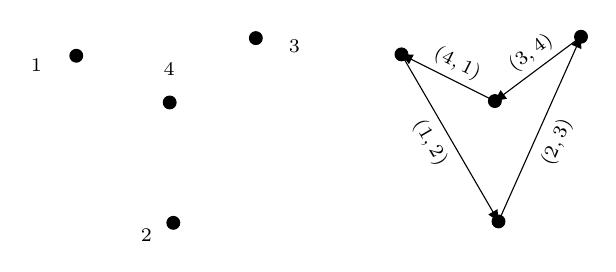
\begin{tikzpicture}[x=0.75pt,y=0.75pt,yscale=-1,xscale=1]
%uncomment if require: \path (0,300); %set diagram left start at 0, and has height of 300

%Shape: Circle [id:dp8468581866061076] 
\draw  [fill={rgb, 255:red, 0; green, 0; blue, 0 }  ,fill opacity=1 ] (129.75,151.67) .. controls (129.75,149.98) and (131.13,148.6) .. (132.83,148.6) .. controls (134.52,148.6) and (135.9,149.98) .. (135.9,151.67) .. controls (135.9,153.37) and (134.52,154.75) .. (132.83,154.75) .. controls (131.13,154.75) and (129.75,153.37) .. (129.75,151.67) -- cycle ;
%Shape: Circle [id:dp1092279369277932] 
\draw  [fill={rgb, 255:red, 0; green, 0; blue, 0 }  ,fill opacity=1 ] (131.5,209.67) .. controls (131.5,207.98) and (132.88,206.6) .. (134.58,206.6) .. controls (136.27,206.6) and (137.65,207.98) .. (137.65,209.67) .. controls (137.65,211.37) and (136.27,212.75) .. (134.58,212.75) .. controls (132.88,212.75) and (131.5,211.37) .. (131.5,209.67) -- cycle ;
%Shape: Circle [id:dp47847609424251114] 
\draw  [fill={rgb, 255:red, 0; green, 0; blue, 0 }  ,fill opacity=1 ] (171.25,120.67) .. controls (171.25,118.98) and (172.63,117.6) .. (174.33,117.6) .. controls (176.02,117.6) and (177.4,118.98) .. (177.4,120.67) .. controls (177.4,122.37) and (176.02,123.75) .. (174.33,123.75) .. controls (172.63,123.75) and (171.25,122.37) .. (171.25,120.67) -- cycle ;
%Shape: Circle [id:dp13281179663837128] 
\draw  [fill={rgb, 255:red, 0; green, 0; blue, 0 }  ,fill opacity=1 ] (84.75,129.17) .. controls (84.75,127.48) and (86.13,126.1) .. (87.83,126.1) .. controls (89.52,126.1) and (90.9,127.48) .. (90.9,129.17) .. controls (90.9,130.87) and (89.52,132.25) .. (87.83,132.25) .. controls (86.13,132.25) and (84.75,130.87) .. (84.75,129.17) -- cycle ;
%Shape: Circle [id:dp9047785488054659] 
\draw  [fill={rgb, 255:red, 0; green, 0; blue, 0 }  ,fill opacity=1 ] (286.42,151.01) .. controls (286.42,149.31) and (287.79,147.93) .. (289.49,147.93) .. controls (291.19,147.93) and (292.57,149.31) .. (292.57,151.01) .. controls (292.57,152.71) and (291.19,154.08) .. (289.49,154.08) .. controls (287.79,154.08) and (286.42,152.71) .. (286.42,151.01) -- cycle ;
%Shape: Circle [id:dp4512249144398415] 
\draw  [fill={rgb, 255:red, 0; green, 0; blue, 0 }  ,fill opacity=1 ] (288.17,209.01) .. controls (288.17,207.31) and (289.54,205.93) .. (291.24,205.93) .. controls (292.94,205.93) and (294.32,207.31) .. (294.32,209.01) .. controls (294.32,210.71) and (292.94,212.08) .. (291.24,212.08) .. controls (289.54,212.08) and (288.17,210.71) .. (288.17,209.01) -- cycle ;
%Shape: Circle [id:dp7255085919283367] 
\draw  [fill={rgb, 255:red, 0; green, 0; blue, 0 }  ,fill opacity=1 ] (327.92,120.01) .. controls (327.92,118.31) and (329.29,116.93) .. (330.99,116.93) .. controls (332.69,116.93) and (334.07,118.31) .. (334.07,120.01) .. controls (334.07,121.71) and (332.69,123.08) .. (330.99,123.08) .. controls (329.29,123.08) and (327.92,121.71) .. (327.92,120.01) -- cycle ;
%Shape: Circle [id:dp7940275676020767] 
\draw  [fill={rgb, 255:red, 0; green, 0; blue, 0 }  ,fill opacity=1 ] (241.42,128.51) .. controls (241.42,126.81) and (242.79,125.43) .. (244.49,125.43) .. controls (246.19,125.43) and (247.57,126.81) .. (247.57,128.51) .. controls (247.57,130.21) and (246.19,131.58) .. (244.49,131.58) .. controls (242.79,131.58) and (241.42,130.21) .. (241.42,128.51) -- cycle ;
%Straight Lines [id:da7630243708026373] 
\draw    (244.49,128.51) -- (289.74,206.41) ;
\draw [shift={(291.24,209.01)}, rotate = 239.85] [fill={rgb, 255:red, 0; green, 0; blue, 0 }  ][line width=0.08]  [draw opacity=0] (5.36,-2.57) -- (0,0) -- (5.36,2.57) -- cycle    ;
%Straight Lines [id:da7466547663908568] 
\draw    (291.24,209.01) -- (329.77,122.75) ;
\draw [shift={(330.99,120.01)}, rotate = 114.07] [fill={rgb, 255:red, 0; green, 0; blue, 0 }  ][line width=0.08]  [draw opacity=0] (5.36,-2.57) -- (0,0) -- (5.36,2.57) -- cycle    ;
%Straight Lines [id:da5263162246336347] 
\draw    (330.99,120.01) -- (291.9,149.21) ;
\draw [shift={(289.49,151.01)}, rotate = 323.24] [fill={rgb, 255:red, 0; green, 0; blue, 0 }  ][line width=0.08]  [draw opacity=0] (5.36,-2.57) -- (0,0) -- (5.36,2.57) -- cycle    ;
%Straight Lines [id:da700113901084908] 
\draw    (289.49,151.01) -- (247.17,129.85) ;
\draw [shift={(244.49,128.51)}, rotate = 26.57] [fill={rgb, 255:red, 0; green, 0; blue, 0 }  ][line width=0.08]  [draw opacity=0] (5.36,-2.57) -- (0,0) -- (5.36,2.57) -- cycle    ;

% Text Node
\draw (64.67,129.6) node [anchor=north west][inner sep=0.75pt]  [font=\scriptsize] [align=left] {$\displaystyle 1$};
% Text Node
\draw (117.67,211.27) node [anchor=north west][inner sep=0.75pt]  [font=\scriptsize] [align=left] {$\displaystyle 2$};
% Text Node
\draw (189,120.27) node [anchor=north west][inner sep=0.75pt]  [font=\scriptsize] [align=left] {$\displaystyle 3$};
% Text Node
\draw (128.67,131.27) node [anchor=north west][inner sep=0.75pt]  [font=\scriptsize] [align=left] {$\displaystyle 4$};
% Text Node
\draw (256.73,156.68) node [anchor=north west][inner sep=0.75pt]  [font=\scriptsize,rotate=-59.54] [align=left] {$\displaystyle ( 1,2)$};
% Text Node
\draw (308.71,180.59) node [anchor=north west][inner sep=0.75pt]  [font=\scriptsize,rotate=-293.67] [align=left] {$\displaystyle ( 2,3)$};
% Text Node
\draw (292.72,131.06) node [anchor=north west][inner sep=0.75pt]  [font=\scriptsize,rotate=-323.41] [align=left] {$\displaystyle ( 3,4)$};
% Text Node
\draw (262.25,121.79) node [anchor=north west][inner sep=0.75pt]  [font=\scriptsize,rotate=-26.71] [align=left] {$\displaystyle ( 4,1)$};


\end{tikzpicture}

    \caption{Example of the Planar Straight Line Graph (PSLG) that defines a dart-like polygon. PSLGs are collections of points and segments that define the polygon's boundary.}
    \label{fig:pslg}
\end{figure}

To do this, the section of the volume is extracted at the minimum \textit{z}-value to obtain all the perimeters present.
These perimeters will correspond to the boundaries that have to be defined and input to the triangulation function.
Once the section is obtained, it is divided by the connected components and the number of points of each component is simplified by merging collinear segments\footnote{\label{footnote:simplify}Trimesh's \href{https://trimesh.org/trimesh.path.path.html\#trimesh.path.path.Path2D.simplify}{simplify} function is used.} to avoid an excess of points in the boundary. 
Finally, the resulting points are iterated, and the index of each point is paired with the next one, obtaining the segments that define each of the boundaries present in the volume.

An example of this procedure is shown in \textcolor{blue}{Figure} \ref{fig:reduction}.
In the \textcolor{blue}{Figure} \ref{fig:reduction} \textcolor{blue}{A} the points retrieved from the section at \textit{z}-minimum value are shown. 
Also, coloured depending on whether they are points from the outer mesh or the inner meshes.
It can be seen that all sections are composed of many points and that it is necessary to reduce the number of points.
After removing all the collinear segments, the number of points is reduced as shown in the \textcolor{blue}{Figure} \ref{fig:reduction} \textcolor{blue}{B}.
As the outer perimeter is rectangular, almost all its segments are collinear.
So, the only remaining points are the ones at each corner.
However, the inner perimeters are circles, so they do not have collinear segments. 
Therefore, to reduce the number of points, they are replaced by circular paths composed of fewer points. 
The function used\footref{footnote:simplify} allows controlling the tolerance between the replaced circle and the resulting circle. 
The greater the tolerance, the lower the final number of points.


\begin{figure}[!htbp]
    \centering
    \begin{subfigure}[b]{0.49\textwidth}
        \centering
        \\includegraphics[width=\textwidth]{imgs/before_reduction.svg.pdf}
        \caption{Points obtained from the section of the volume}
    \end{subfigure}
    \begin{subfigure}[b]{0.49\textwidth}
        \centering
        \\includegraphics[width=\textwidth]{imgs/after_reduction.svg.pdf}
        \caption{Reduction of the collinear points and circular paths.}
    \end{subfigure}
    \caption{Example of points reduction. Image \textbf{A} shows the initial points obtained from the section of the volume. Image \textbf{B} shows the resulting points from removing all the collinear points and substituting the circles with circular paths composed of fewer points.}
    \label{fig:reduction}
\end{figure}

\subsection{Initial layer tessellation}

Once all the different contours are defined, the surface can be tessellated using \textit{Triangle}.
To do so, the function \textit{triangulate} is used.
This function requires a Python dictionary as input, which gathers the information about the vertices, segments and holes under three keys with these same names.
A 2D-array that stores the \textit{xy} position of each vertex is passed in the \textit{vertices} key. 
The segments obtained in the above-mentioned process are stored in the \textit{segments} key. 
And, finally, the key \textit{holes} stores a 2D-array containing a point inside each hole. 
In this case, the centre of each hole is used, obtained by calculating the mean \textit{xy} position of all the points that compose the boundary of each hole.

Additionally, the function allows tuning the tessellation by passing an optional \textit{string} as a second argument.
This \textit{string} can be composed by multiple parameters\footnote{There are many parameters available, each with different purposes. 
This work will only mention the parameters used, but readers are encouraged to read the \href{https://www.cs.cmu.edu/~quake/triangle.switch.html}{\textit{Command line switches}} section available on the official website of this package for better and more information about the available commands.
} to bias the behaviour of the tessellation engine.
If the purpose of using this package is merely to triangulate a set of points, the use of these optional parameters is not necessary. 
However, if it is necessary to impose any restrictions on the triangulation, it may be necessary to use some of them. 
Setting boundaries is a restriction in itself, and therefore, it is necessary to use some parameters to delimit the triangulation to the surface of interest at any given time.
The following parameters are used in this work:

\begin{itemize}
    \item \textit{-p}: It is used to tessellate a PSLG, i.e., when the triangulation is to be restricted to a domain defined by boundaries. Needed if the key \textit{segments} is input.
    \item \textit{-q}: Quality mesh generation with no angles smaller than 20 degrees. An alternate minimum angle may be specified after the \textit{q}.
    \item \textit{-a}: Imposes a maximum triangle area constraint. A fixed area constraint, that applies to every triangle, may be specified after the \textit{a}.
\end{itemize}

When using constraints, such as quality mesh (\textit{-q}) or maximum area (\textit{-a}), during the triangulation, the use of Stainer points\footnote{In computational geometry, a Steiner point is a point that is not part of the input to a geometric optimization problem but is added during the solution of the problem, to create a better solution than would be possible from the original points alone.} is considered by the engine.
Those points are needed sometimes to guarantee the imposed constraints.
Far from being a drawback, this feature is essential to generate the initial layer tessellation.
As stated in the definition of the problem at the beginning of this manuscript, controlling pore size is one of the objectives sought with this methodology.
In the \textcolor{blue}{Figure} \ref{fig:reduction} can be seen that at this point only a set of contours is disposed. 
Using Stainer points and area restriction, it is possible to fill the initial surface with the necessary number of points to ensure that the average area of the initial triangles is equal to the defined pore size.
Since the maximum area value set with the parameter \textit{-a} to the triangulation function is not directly related to the desired pore size, it is necessary to find the value that generates the tessellation whose average triangle area value is equal to the desired value.
To do this, a binary search is performed in the interval $[pore\_size/10, pore\_size*10]$. 
At each step, a tessellation is generated with a maximum area restriction equal to the midpoint of the search interval, and the average area of all triangles is calculated. 
To ensure convergence of the search, a tolerance of 5\% of the searched pore size is allowed. 
Also, a maximum of 50 iterations is set to find the desired value. 
This is done in order to avoid infinite loops, since not any pore size can be obtained. 
There will always be a maximum pore size limit that can be reached, which will depend on the topology in each case. 
The parameter \textit{-q} is also used to obtain more regular triangles to obtain more uniform tetrahedra in the first layer.
In the \textcolor{blue}{Figure} \ref{fig:first_layer_hole}, two examples of the tessellations obtained from the section in \textcolor{blue}{Figure} \ref{fig:reduction} \textcolor{blue}{B} and a pore area of 80 $mm^{2}$ and 50 $mm^{2}$ respectively are shown.


\begin{figure}[!htbp]
    \centering
    \begin{subfigure}[b]{0.49\textwidth}
        \centering
        \\includegraphics[width=\textwidth]{imgs/first_layer_hole_tess.svg.pdf}
        \caption{Pore area = 80 $mm^{2}$}
    \end{subfigure}
    \begin{subfigure}[b]{0.49\textwidth}
        \centering
        \\includegraphics[width=\textwidth]{imgs/first_layer_hole_50.svg.pdf}
        \caption{Pore area = 50 $ mm^{2}$}
    \end{subfigure}
    \caption{Example of \textcolor{blue}{Figure} \ref{fig:reduction} \textcolor{blue}{B}  section tessellation. Image \textbf{A} shows the tessellation obtained with a pore area parameter equal to 80 $ mm^{2}$. Image \textbf{B} shows tessellation obtained with a pore area parameter equal to 50 $mm^{2}$.}
    \label{fig:first_layer_hole}
\end{figure}

Furthermore, to show the effect that the \textit{-q} parameter has on tessellation, a comparison between two tessellations with a pore size of 100 $mm^{2}$ is shown in \textcolor{blue}{Figure} \ref{fig:comp_q}. 
The image shows the points of the initial section (\textcolor{blue}{Figure} \ref{fig:reduction} \textcolor{blue}{B}) that are input into the triangulation function in black, the Steiner points generated by the triangulation routine with the \textit{-q} parameter activated in orange, and the Steiner points generated by the routine with the \textit{-q} parameter deactivated in green. 
In addition, the triangulation that would be obtained with the \textit{-q} parameter deactivated is shown by dotted purple lines. 
It can be seen that in this case, the triangles obtained are mostly obtuse. When the \textit{-q} parameter is activated, they tend to be more acute.

\begin{figure}[!htbp]
    \centering
    \\includegraphics[width =\textwidth]{imgs/q_param_comp.svg.pdf}
    \caption{Comparison between the tessellation obtained when activating or deactivating the \textit{-q} parameter. The initial section points are shown in black, the Steiner points generated by the triangulation routine with the \textit{-q} parameter activated in orange, and the Steiner points generated by the routine with the \textit{-q} parameter deactivated in green. Also, the triangulation that would be obtained with the \textit{-q} parameter deactivated is shown by dotted purple lines. }
    \label{fig:comp_q}
\end{figure}

\section{Generation of the contour segments (TBC)}

In the \textcolor{blue}{Section} \ref{{subsec:shell_struct_connection}}, the methodology used to join the structure and the surface of the volume was explained.
Since the geometries admitted up to that point were merely convex, the outermost generated vertices, the convex hull, could be obtained and projected orthogonally to the surface of the volume. 
Now, the supported geometries include non-convex geometries. 
Therefore, another strategy must be found to project the outer vertices onto the surface of the volume, since it is not possible to calculate the convex hull of this type of structure, as has been proven above. 
Moreover, in case it is possible to obtain the outermost points by calculating the convex hull, because the outer contour is concave, there is no way to find the closest points to the possibly present inner surfaces.
In addition, in each of the layers that make up a structure, the segments that form part of the various contours must be identified to carry out the triangulations.
This section will explain what strategies were followed to overcome each of the two problems.

\subsection{Obtaining the boundary segments}\label{sec:segments}

\textcolor{blue}{Figure} \ref{fig:comp_q} shows an example of triangulation carried out for a surface with several holes. 
In it, the reader can see that the segments introduced to the triangulation function are those formed after joining the black points, obtained after reducing the number of points extracted from the volume section. 
These initial points and segments, together with the pore size, make it possible to obtain the triangulation shown in the figure by adding several Steiner points. 
It can be noticed that several of these Steiner points were added by the engine, in the middle of the segments forming the contour. 
When this happens, the triangulator subdivides these segments in order to add interior points to generate a triangulation that satisfies the imposed conditions. 
This means that the triangulation function itself also returns the segments generated during the triangulation. 
It is therefore possible to retrieve them in order to use them in the following layers. 
Because the vertices generated from tetrahedra whose bases contain one of those segments can be considered as the closest points to the surfaces and, therefore, the ones to be projected.

When the generator adds new segments and points, it does not return them sorted. Therefore, to discern which segments belong to which contour, they have to be grouped together. 
As these are related points belonging to different groups, they can be treated as disjoint sets, so a Find-Union algorithm with path compression was implemented in order to obtain the indices of the points that are part of each of the sections. 
It has been considered of interest to explain how this algorithm works and how it was implemented. 
Therefore, the code fragment developed is shown below, together with a brief example of how it works:



\begin{lstlisting}[style=customdark, caption={Function to group segments using Union-Find with path compression}]
def group_segments(segments):
    parent = {}
    def find(node):
        # Find the representative of the set with path compression
        if parent[node] != node:
            parent[node] = find(parent[node])
        return parent[node]

    def union(node1, node2):
        # Join two roots
        root1 = find(node1)
        root2 = find(node2)
        if root1 != root2:
            parent[root2] = root1

    # Initialise nodes in Union-Find
    for seg in segments:
        for node in seg:
            if node not in parent:
                parent[node] = node

    # Process segments to join components
    for seg in segments:
        union(seg[0], seg[1])

    # Group nodes by component
    groups = {}
    for node in parent:
        root = find(node)
        if root not in groups:
            groups[root] = []
        groups[root].append(node)

    group_list = list(groups.values())

    return group_list

\end{lstlisting}


Let's suppose that the following list of segments is given from the triangulation function and passed to the \texttt{group\_segments()} function:
\[
\texttt{segments = [(1, 2), (2, 3), (4, 5), (5, 6), (7, 8), (9, 10), (10, 11), (3, 4)]}
\]
Each node is initialised to be its own parent:
\[
\texttt{parent = \{1:1, 2:2, 3:3, 4:4, 5:5, 6:6, 7:7, 8:8, 9:9, 10:10, 11:11\}}
\]
Then, the segments are iterated over to perform the joins between each one and its root, in order to relate the nodes with each of the different roots found.
This allows related components to be discovered in a list of relationships.

\begin{itemize}
  \item Union(1, 2) → parent[2] = 1
  \item Union(2, 3) → parent[3] = 1
  \item Union(4, 5) → parent[5] = 4
  \item Union(5, 6) → parent[6] = 4
  \item Union(7, 8) → parent[8] = 7
  \item Union(9, 10) → parent[10] = 9
  \item Union(10, 11) → parent[11] = 9
  \item Union(3, 4) → roots of 3 and 4 are 1 and 4 → parent[4] = 1
\end{itemize}

Initially, without path compression, to find the root of node 6, the following unions should be done:
\[
6 \rightarrow 5 \rightarrow 4 \rightarrow 1
\]
However, path compression updates all the parents at once. After calling \texttt{find(6)}, path compression updates:
\[
\texttt{parent[6] = 1, parent[5] = 1, parent[4] = 1}
\]
So the updated structure is:
\[
6 \rightarrow 1,\quad 5 \rightarrow 1,\quad 4 \rightarrow 1
\]
This ensures that every node on the path to the root is directly connected to it, effectively flattening the tree and drastically reducing the cost of future \texttt{find()} calls. With path compression, the time complexity per operation becomes:

\[
\mathcal{O}(\alpha(n))
\]

where \(\alpha(n)\) is the inverse Ackermann function\footnote{The inverse Ackermann function is the function that returns the pair of integers $(m, n)$ that satisfies the equation $A(m, n) = x$, where $x$ is a given value. It is an extremely slow-growing function which occasionally turns up in computer science and mathematics.}, which is less than 5 for any realistic \(n\).
After processing all unions, nodes 1–6 form one connected component. Nodes 7–8 and 9–11 form their own components. Resulting in the following groups: \texttt{[[1, 2, 3, 4, 5, 6], [7, 8], [9, 10, 11]]}.


\begin{center}
\begin{tikzpicture}[node distance=1.5cm, every node/.style={circle, draw, minimum size=7mm}]
  \node (1) {1};
  \node[right of=1] (2) {2};
  \node[right of=2] (3) {3};
  \node[right of=3] (4) {4};
  \node[right of=4] (5) {5};
  \node[right of=5] (6) {6};

  \node[below=1cm of 2] (7) {7};
  \node[right of=7] (8) {8};

  \node[below=1cm of 5] (9) {9};
  \node[right of=9] (10) {10};
  \node[right of=10] (11) {11};

  \draw (1) -- (2) -- (3) -- (4) -- (5) -- (6);
  \draw (7) -- (8);
  \draw (9) -- (10) -- (11);
\end{tikzpicture}
\end{center}

Once the indices of the points are grouped in lists and sorted depending on their length, the first item on the list will always be the list of points that belong to the outer surface.
So, this list can be split into two to differentiate the outer and inner points.
It is important to have in mind that this needs to be done because the points that will be part of the contours after the triangulation of the initial layer are unknown beforehand.
Only the points that are part of circular contours can be known beforehand in some cases, because Steiner points will rarely be added to the circular boundaries. 
But it depends on the pore size set.
This will help to create the segments for the following layers and identify which points will be projected onto the surface.

\subsection{Surface points identification}

Once triangulation is complete, the tessellation adaptation routine modifies it to obtain the desired number of simplices, and the final list of simplices is obtained. 
For each of these simplices, a tetrahedron is generated in the same way as explained in \textcolor{blue}{Section} \ref{sec:tetrahedra_gen}.

From now on, simplices that contain a boundary segment will be known as "surface simplices" and the points generated from them will be known as "surface points". The reason for grouping surfaces into interior and exterior surfaces is that the exterior surface will always be present, but the interior surfaces may not be present (e.g., a surface without holes) or may even cease to be present throughout the volume (e.g., screw holes). 
Therefore, it is necessary to consider each of the present surfaces individually. 
Hence, when a vertex is created, it is checked whether its base contains at least two points included in any of the surface point lists. 
As the number of interior surfaces is indeterminate, the surface points of each of the detected interior surfaces are stored in a dictionary. 
This dictionary is then looked over to check whether there are at least two points from the base in question that are present in any of them. 
When a base is detected that has two points contained in any of the lists, the search is stopped to improve the efficiency of the algorithm, and the vertex index is saved in the corresponding surface point list.
Before explaining the methodology implemented to identify the surface points of the next layers, the following premises need to be taken into account:

\begin{itemize}
    \item Only one surface point can be generated from each surface simplex.
    \item A surface point will belong to the same surface as its base.
    \item A simplex shall be considered a surface simplex if it contains at least two points of the same surface.
    \item A surface point can belong to several surface simplices. But a pair of surface points can only belong to one surface simplex.
\end{itemize}

Each of these premises will be justified in more depth below:

\subsubsection{Only one surface point can be generated from each surface simplex}

The number of surface simplices cannot increase between layers.
Once the number is simplices per layer is set after the triangulation of the first layer, the maximum number of surface simplices is also defined.
In the following layers, it can only decrease due to they can be merged with neighbouring simplices.
This problem can lead to situations in which the definition of the boundaries is compromised
due to the loss of surface points arising after the union of several surface simplices.
In the \textcolor{blue}{Figure} \ref{fig:cons1}, this issue is illustrated by showing the evolution of the boundary of a bolt hole among the first three layers.
It can be noticed how the number of surface points available to define the bolt's surface decreases in each layer due to the aforementioned problem.
This highlights the need to also control the number of surface simplices in each layer.

\begin{figure}[!htbp]
    \centering
    \begin{subfigure}[b]{0.3\textwidth}
        \centering
        \includegraphics[width=\textwidth]{imgs/cons1_1.png}
        \caption{Initial layer.}
    \end{subfigure}
    \begin{subfigure}[b]{0.3\textwidth}
        \centering
        \includegraphics[width=\textwidth]{imgs/cons1_2.png}
        \caption{Second layer.}
    \end{subfigure}
    \centering
    \begin{subfigure}[b]{0.3\textwidth}
        \centering
        \includegraphics[width=\textwidth]{imgs/cons1_3.png}
        \caption{Third layer.}
    \end{subfigure}
    \caption{Example of surface point loss due to the mixing of surface simplices. From left to right, the definition of the contour of a hole in each of the layers is shown.}
    \label{fig:cons1}
\end{figure}

\subsubsection{A surface point will belong to the same surface as its base}

To maintain the consistency of contours within layers, points generated from a surface simplex must belong to the same surface as the simplex.
Otherwise, the boundaries could become mixed, resulting in a loss of consistency with the initial volume.
This only reinforces the hypothesis that each surface must be analysed individually to find the new points that belong to each one.
Furthermore, another argument to reinforce this hypothesis is based on the fact that there may be situations in which a surface point may be closer to other surfaces than to the one to which it belongs. 
Therefore, if the future projection of these points were carried out as in the previous chapter (projecting the points closest to the surface), surface points assignment errors could occur.
This further justifies the need to analyse surfaces individually. \textcolor{blue}{Figure} \ref{fig:zoomin} shows an example of a situation similar to the one described above. 
It shows a detail of a tessellation in which a point belonging to an interior surface (green) is very close to the exterior surface. 
In the example shown, this problem does not occur, but it serves to show that it is a possible situation.

\begin{figure}[!htbp]
    \centering
    \\includegraphics[width =\textwidth]{imgs/zoomed_inset.svg.pdf}
    \caption{Example of tessellation where the surface points are coloured. Red points are surface points that belong to the outer surface, while green points belong to the different inner surfaces.}
    \label{fig:zoomin}
\end{figure}

\subsubsection{A simplex shall be considered a surface simplex if it contains at least two points of the same surface}

If two surfaces are too close and the pore size is big enough, there can be situations where a surface simplex also contains points that belong to other surfaces.
This only reinforces the need to analyse each surface separately.
Therefore, it is not enough to look for simplices that contain at least two points belonging to the surface to classify a simplex as a surface simplex. 
It is necessary to ensure that at least two points belong to the same surface.
Although this may seem like a very inefficient strategy, it is the only way to ensure that the structure adapts perfectly to the limits of the initial volume.
An example of this situation is shown in the \textcolor{blue}{Figure} \ref{fig:zoomin_2}.
The blank triangle in the detail has two surface points, but since both belong to two different surfaces, this triangle cannot be considered as a surface simplex.

\begin{figure}[!htbp]
    \centering
    \\includegraphics[width =\textwidth]{imgs/zoomed_inset_2.svg.pdf}
    \caption{Example of a simplex containing two surface points that do not belong to the same surface.}
    \label{fig:zoomin_2}
\end{figure}

\subsubsection{A surface point can belong to several surface simplices. But a pair of surface points can only belong to one surface simplex.}

As layers are created, the tessellations become more random, and with them the polygons that compose them. 
These begin to take on unpredictable non-convex shapes.
Some of these non-convex polygons can take on shapes that partially isolate other polygons. 
When this happens to the surface simplices, a situation can arise in which a non-surface simplex contains two points from the same surface and could therefore also be considered a surface simplex. 
An example of this can be seen in \textcolor{blue}{Figure} \ref{fig:zoomin_3}.
As can be seen, the simplex shown in the detail surrounds the surface simplex and contains two points of the surface.
Following the aforementioned criteria, this simplex should be considered as a surface simplex.
But evidently it cannot be, because it is an interior polygon that does not contain any segment of the surface.
Therefore, containing two surface points must be necessary, but not sufficient, to consider a simplex as a surface simplex; these must be consecutive.
A situation could arise in which the polygon shown in the image detail merges with the surface simplex to its right. 
In such a situation, the polygon would contain two consecutive surface points and therefore, once again, could be considered a surface simplex. 
However, once again, it should not be considered as such. 
Therefore, the aforementioned condition must be generalised by establishing that all surface points contained in a simplex must be consecutive.
To solve this, a function was implemented that, given a simplex and all the points on a surface, obtains an array of Booleans where the values will be True if a point is in the list of surface points and False if it is not. 
Then, after binarising this array, it is only necessary to check whether the sequence \textit{010} is present. 
If it is, it means that the simplex has a surface point that is isolated from the others and, therefore, they are not sequential.
For example, the binary number associated with the simplex in the figure would be \textit{1010000} if starting from the leftmost point.
While it is true that the problem of assigning incorrect surface simplices is solved, the proposed solution causes even more loss of contour definition. 
This is because surface simplices that have been joined with other interior simplices may no longer be considered surface simplices, due to the exclusion criterion, creating a gap in the contour.

\begin{figure}[!htbp]
    \centering
    \\includegraphics[width =\textwidth]{imgs/zoomed_3.svg.pdf}
    \caption{Example of a tessellation containing a detailed polygon which contains two surface points but cannot be considered as a surface simplex.}
    \label{fig:zoomin_3}
\end{figure}

As the reader can deduce, the four premises outlined above are the result of problems encountered during the development of this work and which had to be resolved. 
If one pays attention, a common factor can be deduced among all these problems: when including the surface simplices arising from triangulation, they can be modified during the tessellation modification process. 
If it is ensured that simplices containing surface segments are not merged with other simplices, the number of simplices will remain constant across all layers, preventing the delineation of the contours from deteriorating. 
Furthermore, these would be the only simplices that could be considered surface simplices. 
Eliminating simplices containing contour segments before the simplex joining process resolves all of the problems outlined above.
Therefore, from now on, after triangulation, all triangles containing two points from any surface will be detected and removed from the set of triangles. 
This prevents them from being selected during the joining process. 
Once the simplices joining process is complete, all removed triangles will be added back. 
To ensure that the number of simplices at the end of the process remains as desired, the number of simplices to be joined will be equal to the final target number of simplices minus the number of surface simplices removed. 
This maintains the number of simplices throughout the layers.
In the \textcolor{blue}{Figure} \ref{fig:no_triang} \textcolor{blue}{A}, an example of what a triangulation would look like after the surface triangles have been removed is shown. 
The remaining triangles are then processed by the merging routine. 
The isolated points belong to triangles whose vertices are contained in surfaces, and the fact that they are isolated does not affect the merging process.
As can be seen in the \textcolor{blue}{Figure} \ref{fig:no_triang} \textcolor{blue}{B}.
The following section will explain why the corners of the outer contour do not appear in the image.
As a result of this new consideration, the final structure created more faithfully reproduces the surface of the initial volume, as will be shown in forthcoming chapters.
In addition, it is worth mentioning that these modifications do not affect the performance of the methodology for geometries without holes.

\begin{figure}[!htbp]
    \centering
    \begin{subfigure}[b]{0.49\textwidth}
        \centering
        \\includegraphics[width=\textwidth]{imgs/triang_without_surface_simp.svg.pdf}
        \caption{Triangulation after removing the triangles that contain a segment of any surface}
    \end{subfigure}
    \begin{subfigure}[b]{0.49\textwidth}
        \centering
        \\includegraphics[width=\textwidth]{imgs/no_triang_final.svg.pdf}
        \caption{Tessellation obtained after the merging process and adding the surface triangles}
    \end{subfigure}
    \caption{Example of tessellation obtained without considering the surface triangles during the merging process. Image \textbf{A} shows the triangulation input to the merging process, which does not contain the surface triangles. Image \textbf{B} shows the tessellation obtained from the merging process after adding the discarded triangles.}
    \label{fig:no_triang}
\end{figure}

The procedure explained so far for detecting vertices that may be surface points is only valid as long as the generated vertices are within the volume. 
In the last layers, where vertices begin to be generated outside the volume, this task becomes much more complicated.

In the \textcolor{blue}{Section} \ref{sec:termination_cond}, the strategy followed in the last layers to achieve layer construction, even though certain vertices have been generated outside the volume, is explained. 
It is mentioned that when a base generated a vertex outside the volume, it was not added, but rather the base. 
The strategy remains the same, but the procedure becomes more complicated when dealing with non-convex geometries because the surface points must be identified at all times to construct the edge segments.

To assemble the segments, the indices of these points in the complete list of vertices are needed.
When a base generates a valid vertex, this process is simple because the index of that vertex will be the same as that of the base in the list of simplices. T
This is possible because each base generates a point.
But in this case, when a vertex is generated outside the volume, \textit{n} points are added to the list of points for the next iteration (list of vertices). 
\textit{n} is the number of points in the base that are valid to add. 
A point will be valid when it has not been previously added to the vertex list. 
Once the valid points from the base have been filtered, it is checked whether any of them are surface points. 
If there is a valid point from the base that is a surface point, its position in the list of points from the base is retrieved and the following value is added to the index list: \textit{position in the base list + length of the index list}. 
This is repeated for all surface points to be added. 
The reason behind this is that \textit{n} points will be added to the vertex list, but of those \textit{n}, only \textit{m} are surface points that will have to be taken into account in the index list.
To facilitate understanding of this procedure, an example is provided below:

Suppose a base is composed of 5 points:

\[
P = [p_0,\, p_1,\, p_2,\, p_3,\, p_4]
\]

Let the current length of the global vertex list be $N = 120$. 
During this iteration, 4 of the 5 base points are valid to be added as new vertices: $p_0$, $p_1$, $p_2$, and $p_4$. 
Each valid point is appended to the vertex list, so their corresponding global indices will be:

\[
\text{Global indices of valid points: } [120,\, 121,\, 122,\, 123]
\]

Suppose now that only $p_0$ and $p_2$ are surface points. 
To determine which of the added points should be considered to build the boundary segments, their position in the base list (positions $0$ and $2$) is retrieved and the current length of the index list (which is $120$) is added to obtain their global indices:

\[
\text{Surface indices: } [0 + 120,\, 2 + 120] = [120,\, 122]
\]

Therefore, only these two indices are added to the index list used for segment construction. The rest of the valid points are added to the geometry but are not used to form segments at this stage.

\subsection{Joining surface points to surfaces}

Once the process explained in the previous section is completed, a list of vertices is obtained, containing the points that will form part of the next layer and need to be tessellated; a list of indices is generated, containing the indices of the vertices that correspond to the surface points of the outer surface; and a dictionary is created, which stores the list of indices of the vertices that make up each of the inner surfaces.
The next step is the last step to be performed during the process of generating each of the layers.
This is to project the points corresponding to each of the surfaces to adapt the structure to the initial volume.

As has been repeated several times above, each surface must be processed individually. 
To project the points onto the corresponding surface, the surfaces must also be processed individually. 
The outer surface will never be a problem because it will always be present, but the inner surfaces may disappear. 
Therefore, during this process, it will be necessary to check whether the interior surfaces are still present in each of the layers. 
If a surface is still present in a section, it will be considered to be still alive. 
Otherwise, it will be considered dead. 
Therefore, during this process, two tasks will be performed: checking whether the surfaces are still alive and projecting the surface points if they are.
As the outer surface will always be present, there is no need to check whether it is present. 
Its processing will consist of only one task, which is to orthogonally project the surface points corresponding to the outer surface onto that surface. 
To do this, the surface point with the shortest distance from each of them is calculated.
Concerning interior surfaces, the logic implemented below will only be processed if interior surfaces exist. 
Thus, the implemented function is generalised for geometries with and without holes.

If there are interior surfaces, a dictionary containing the list of surface point indices for each of the surfaces shall be provided. 
Besides the list of meshes containing the inner surface meshes.
The first problem arises because this dictionary is not ordered. 
As this dictionary is generated as each of the bases extracted from the modified tessellation is processed, it is not possible to control the order in which these bases are processed. 
That is why the keys in the dictionary are only the index in the order in which each of the surfaces is detected and bear no relation to any geometric aspect of them. 
Therefore, each time a key in the dictionary is iterated, it is not known to which surface it corresponds. 
So the first step will be to identify which surface each entry in the dictionary corresponds to.

To link the dictionary entries to each of the surfaces, both objects are traversed in a nested manner. 
For each key in the dictionary, the list of meshes is iterated to find out which one it corresponds to. 
As each key in the dictionary has an associated value that corresponds to the indices of the vertices that correspond to the surface points of each of the detected surfaces, these points can be retrieved, and the centroid of the set can be calculated. 
Then, the centroid of each mesh that corresponds to the centroid of the points is sought, taking into account a certain tolerance. 
If two centroids coincide, it means that the points of that key correspond to the surface pointed at that moment. 
Once this is done, the coordinates of each of the surface points are retrieved and their projection onto the surface is calculated. 

As mentioned above, the orthogonal projection will be the point with the shortest distance between the point in question and the surface. 
If a surface point has exceeded its corresponding mesh, i.e., is above it, its orthogonal projection will be a point located at the upper limit of the mesh. 
If this happens, that point will be counted as a dead point. 
If half of the surface points are dead points, that mesh will be considered dead and should no longer be taken into account. 
A representative number of dead points is necessary to consider a mesh dead because tetrahedra do not grow at the same rate, and there may be areas adjacent to a hole where taller tetrahedra are generated. 
However, the fact that one point has exceeded the mesh does not imply that the rest have and therefore must be eliminated. 
In addition, a 1 cm margin was added to consider a point as having exceeded a mesh and should be declared a dead point.
Once all dictionary entries have been processed, all dead meshes and their corresponding dictionary entries will be removed so that they will not be part of the surface segments in the next triangulation.
Thanks to this process, each layer can be rigorously adapted to the internal geometry of each volume. Once each point has been projected to the proper surface, the boundary segments to tessellate the following layer can be obtained as explained in \textcolor{blue}{Section} \ref{sec:segments}.

This method has one unavoidable drawback. 
If the workpiece has a rectangular shape, its corners cannot be mapped and will be lost (\textcolor{blue}{Figure} \ref{fig:zoomin_3})
This is because the orthogonal projection of the points generated in the corner tetrahedra will never lie on the corners. 
To maintain the original shape, points would have to be forced to appear at the corners. 
But this poses two problems. The first is that adding points that are not part of the originals would cause them to float in space, without continuity, since they do not arise from previous ones. 
The second is that it is not possible to know in general what the shape of the volume is and whether or not points need to be added at the corners.
Therefore, adding a routine that forces the appearance of points at the corners would lead to two new problems: having to define and characterise what is considered a corner and the possible accumulation of points, which could be counterproductive. 
Therefore, it was decided that accepting the loss of the corners is the best solution, despite the loss of fidelity to the original volume.

\section{Growth vector conditioning}

\textcolor{blue}{Section} \ref{sec:tetrahedra_gen} introduces the concept of growth vector. 
This vector allows the direction of growth of the tetrahedra to be conditioned to adapt to inclined or conical geometries. 
Depending on the distance of the tetrahedron from the centre of the section and its height, the vector will have a greater or lesser slope.
Growth vectors in conical geometries, for example, are completely vertical if their base is located at the centre of the section and are parallel to the external surface if they are generated from surface simplices.
Therefore, the simplices between these cases will generate growth vectors with a gradient in the inclination between these two cases.
\textcolor{blue}{Figure} \ref{fig:gv_cond_1} illustrates an example of this gradient of growth vector inclinations in a section of a conical volume. 
Due to radial symmetry, only vectors between $r=0$ and $r=R$ are shown.

\begin{figure}[!htbp]
    \centering
    \\includegraphics[width =0.9\textwidth]{imgs/gv_1.svg.pdf}
    \caption{Example of the distribution of growth vectors among a conical section.}
    \label{fig:gv_cond_1}
\end{figure}

Volumes containing holes cannot use this growth vector definition, as they have areas without material that should not be taken into account when calculating the growth vector slope. 
For example, suppose an annular section with an inner radius $R_1$ and an outer radius $R_2$, as shown in \textcolor{blue}{Figure} \ref{fig:gv_cond_2}. 
According to the current definition of growth vector, the vectors from the surface simplices of the inner surface will generate vertices outside the volume, since their growth vectors point towards the centre of the volume, which is not within the domain of the volume.
It can be noticed, in the figure, that the innermost vector begins inside the volume but ends outside it. 
In that case, the vertex generated by this vector would be outside the volume.

\begin{figure}[!htbp]
    \centering
    \\includegraphics[width =0.9\textwidth]{imgs/gv_2.svg.pdf}
    \caption{Example of distribution of growth vector along a annular section. Straight line represents the outer surface while dashed line represents the inner surface. Gray vectors represent the vectors that  would lie outside the volume.}
    \label{fig:gv_cond_2}
\end{figure}

Therefore, the growth vectors of inner surface simplices should be parallel to those surfaces, regardless of their position. 
Then, in a hollow volume, the growth vectors have to have inclinations that vary between the inclination of the inner surface and the inclination of the outer surface, as shown in \textcolor{blue}{Figure} \ref{fig:gv_cond_3}.
It should be noted that this figure was obtained by varying the angle of an equispaced vector along the section, but it is not a possible solution to the problem posed. 
It has only been added as visual support.

\begin{figure}[!htbp]
    \centering
    \\includegraphics[width =0.9\textwidth]{imgs/gv_3.svg.pdf}
    \caption{Example of a linear growth vectors distribution along a annular section.}
    \label{fig:gv_cond_3}
\end{figure}

To solve this, the growth vector is multiplied by a slope adjustment constant, $\alpha \in [0,1]$, so that the vectors are more vertical the closer they are to the inner surface and take their original value near the outer surface. 
It was decided to use a sigmoid function to define this constant, rather than a linear function, to obtain areas of little variation in slope near each of the extremes.
Specifically, a hyperbolic tangent function adjusted to the interval [0,1] was used (\textcolor{blue}{Equation} \ref{eq:tanh}), to which a value \textit{k} was added to modify the slope. 
To calculate $\alpha$, the inner and outer radius values of the section are first calculated, and then the relative position of the base with respect to the midpoint of both limits is normalised. 

\begin{equation}\label{eq:tanh}
    \alpha(x,k) = \frac{1}{2}\left( \tanh\left( k\cdot\frac{x -\left(outer\:radius + inner\:radius  \right)/2}{outer\:radius - inner\:radius} \right) +1 \right)
\end{equation}

\textcolor{blue}{Figure} \ref{fig:alpha} shows an example of how the value \textit{k} affects the slope of the function. 
For this purpose, values of $R_1 = 5$ cm and $R_2 = 10$ cm have been used. 

\begin{figure}[!htbp]
    \centering
    \includegraphics[width =0.7\textwidth]{imgs/alpha.png}
    \caption{Comparison of \textcolor{blue}{Equation} \ref{eq:tanh} for different values of $k$ in the interval [5,10] cm.}
    \label{fig:alpha}
\end{figure}

In this work, a value of $k=5$ has been used, as this yields a function that allows the alpha value to be practically constant in the vicinity of the extremes and also achieves a smooth slope. 
However, this value is fully customisable.
\textcolor{blue}{Figure} \ref{fig:gv_cond_4} shows how this factor affects to the growth vector along an annular section.
By doing this, the vectors near the surfaces tend to be parallel to them while suffering a smooth transition in the middle.

\begin{figure}[!htbp]
    \centering
    \\includegraphics[width =0.9\textwidth]{imgs/gv_4.svg.pdf}
    \caption{Example of growth vector distribution utilising the adjustment parameter $\alpha$ to modify the inclination. In this example, a parameter $k=5$ was used.}
    \label{fig:gv_cond_4}
\end{figure}

\end{document}

